This section presents the results obtained by coding the messages with codes having the same code rate (in our case 1/2) but different constraint lengths. Figure \ref{fig:constantCodeRateRandomFigure} indicates that having a higher constraint length reduced the number of decoded errors. However, this is true only for relatively small channel error rates. It can be seen in figure \ref{fig:constantCodeRateRandomFigure} that for our examples, the code with the highest constraint length starts to perform worse than the other at a channel error rate close to 0.08. 
The results of the simulation performed using a channel that introduces bursts errors are shown in figures \ref{fig:constantCodeRateBurstFigure} and \ref{fig:constantCodeRateMarkovFigure}. \todo{Continue here}


\begin{figure}
\centering
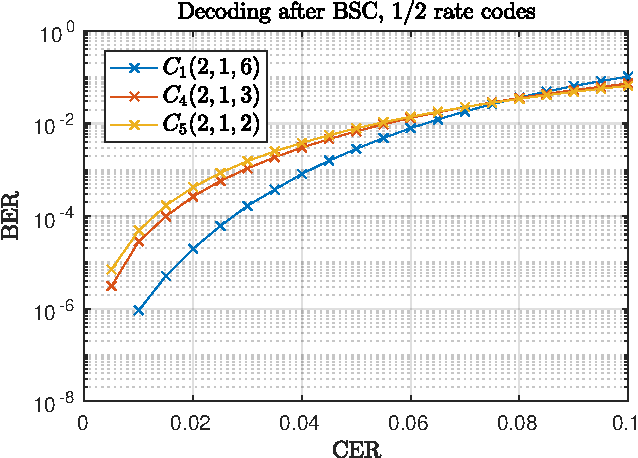
\includegraphics[scale=1]{../figures/extra12rand.pdf} 
\caption{1/2 rate\todo[inline]{change caption}\label{fig:constantCodeRateRandomFigure}}
\end{figure}

\begin{figure}
\centering
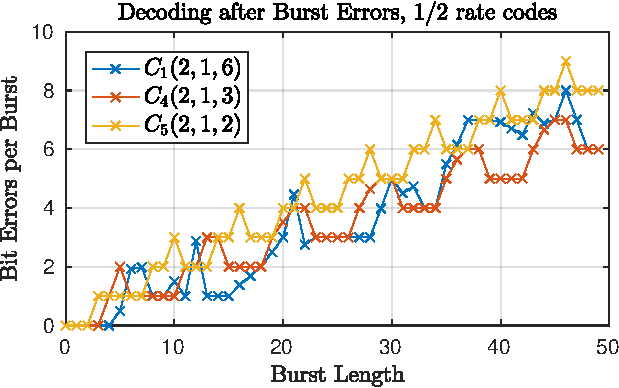
\includegraphics[scale=1]{../figures/extra12burst.pdf} 
\caption{1/2 rate\todo[inline]{change caption}\label{fig:constantCodeRateBurstFigure}}
\end{figure}

\begin{figure}
\centering
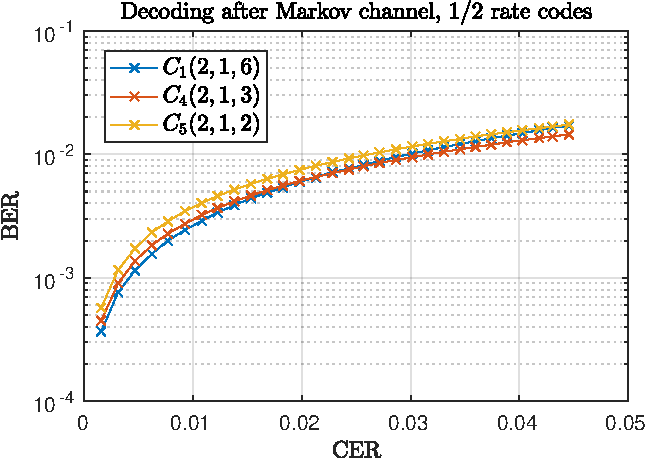
\includegraphics[scale=1]{../figures/extra12markov.pdf} 
\caption{1/2 rate\todo[inline]{change caption}\label{fig:constantCodeRateMarkovFigure}}
\end{figure}